\documentclass{beamer}
\usetheme[pageofpages=of,% String used between the current page and the
                         % total page count.
          bullet=circle,% Use circles instead of squares for bullets.
          titleline=true,% Show a line below the frame title.
          alternativetitlepage=true,% Use the fancy title page.
       %   titlepagelogo=logo-polito,% Logo for the first page.
       %   watermark=watermark-polito,% Watermark used in every page.
       %   watermarkheight=100px,% Height of the watermark.
       %   watermarkheightmult=4,% The watermark image is 4 times bigger
                                % than watermarkheight.
          ]{Torino}

\setbeamertemplate{footline}{
  \begin{beamercolorbox}[wd=\paperwidth,ht=1ex,dp=1ex]{footline}
    \vspace{5pt} \hspace{1em} \insertframenumber/\inserttotalframenumber
  \end{beamercolorbox}
}

\author{Brendon J. Brewer}
\title{STATS 331 -- Introduction to Bayesian Statistics}
\institute{The University of Auckland}
\date{}


\linespread{1.3}
\usepackage{minted}
\usepackage[utf8]{inputenc}
\usepackage{dsfont}
\newcommand{\given}{\,|\,}
\newcommand{\balpha}{\boldsymbol{\alpha}}
\newcommand{\bmu}{\boldsymbol{\mu}}


\begin{document}

\frame{\titlepage}

\begin{frame}
\begin{center}
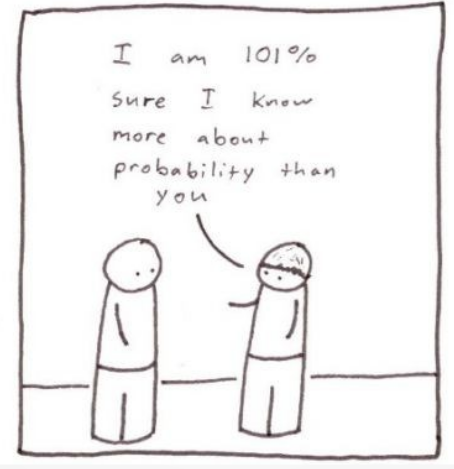
\includegraphics[width=0.6\textwidth]{images/101.png}

Credit: www.afewpanels.com
\end{center}

\end{frame}


\begin{frame}
\Large

\begin{center}
Time Series Models
\end{center}
\end{frame}

\begin{frame}
\frametitle{Poll}
How many of you have studied a course involving `time series models'
such as the AR(1)?
\end{frame}


\begin{frame}
\frametitle{What is a Time Series}
There are two related meanings for the term {\bf time series}.

\begin{itemize}
\item [(1)] Any quantity that varies over time.
\end{itemize}

\begin{center}
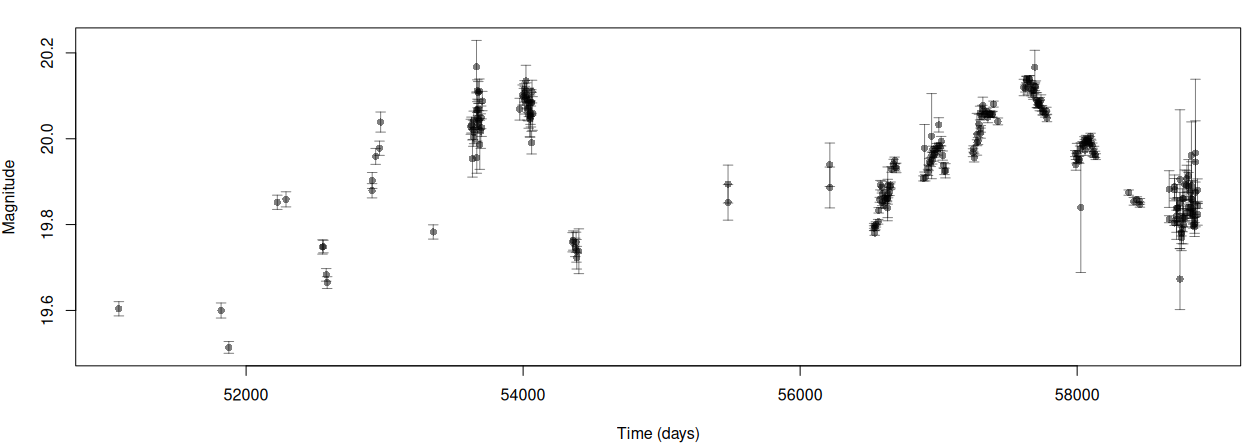
\includegraphics[width=0.9\textwidth]{images/time_series.png}
\end{center}

\end{frame}

\begin{frame}
\frametitle{What is a Time Series}
There are two related meanings for the term {\bf time series}.

\begin{itemize}
\item [(2)] A {\bf probability distribution} for a quantity that varies over time.\pause
\item That is, not any single curve, but a probability distribution over the
set of possible curves.
\end{itemize}

\end{frame}


\begin{frame}
\frametitle{Time Series Models}
Time series models are heavily used in finance, but are also used in a 
variety of other fields (e.g., the previous plot was astronomy data).

\end{frame}

\begin{frame}
\frametitle{The AR(1) Model}

\begin{itemize}
\item In STATS 331 we will only study the AR(1) model, which is a relatively simple
time series model. The AR stands for auto-regressive.\pause
\item It is a probability distribution for the values $y_1, y_2, y_3, ...$
of a series at times $t=1, 2, ...$.
Time is {\bf discrete} and there are {\bf no gaps}.\pause
\item Remember, no single curve $(y_1, y_2, y_3, ...)$ is an AR(1), it is
the probability distribution for the curve that is AR(1).\pause
\item The AR(1) might be a prior distribution or a sampling distribution
depending on the application. For us, it will be the latter.
\end{itemize}
\end{frame}

\begin{frame}
\frametitle{The AR(1) Model}

\begin{itemize}
\item The value of the quantity $y_{t+1}$ at the next timestep is given by
a function of the current value $y_{t}$ plus an `innovation'.\pause
\item We only specify a probability distribution for the innovations.\pause
\end{itemize}
\begin{align}
y_{t+1} &= \mu + \alpha(y_t - \mu) + \epsilon_t \\
\epsilon_t \given \beta &\sim \textnormal{Normal}(0, \beta^2).
\end{align}

\end{frame}


\begin{frame}
\frametitle{The AR(1) Model: Parameters}
In the previous equations we introduced the
three parameters of the AR(1) model:\pause
\begin{itemize}
\item $\mu$ describes the mean level that the $y$s fluctuate around.\pause
\item $\alpha$ describes how strongly the next value $y_{t+1}$ is influenced
by the current value $y_t$. It is usually between 0 and 1.\pause
\item $\beta$ describes the typical size of the innovations.
\end{itemize}

\end{frame}


\begin{frame}
\frametitle{Thinking About the AR(1)}
If we set $\beta$ to zero, the AR(1) process becomes deterministic and
describes an exponential decay towards $\mu$. The speed of the decay is
controlled by $\alpha$.
\begin{align}
y_{t+1} &= \mu + \alpha(y_t - \mu)
\end{align}

\end{frame}


\begin{frame}[fragile]
\frametitle{Simulating an AR(1) in R}
\begin{minted}{r}
N = 1000       # Length of simulation
mu = 5.0       # Parameters
alpha = 0.99
beta = 1
y = numeric(N) # Storage
for(i in 1:(N-1))
{
    y[i+1] = mu + alpha*(y[i] - mu) + beta*rnorm(1)
}
\end{minted}

\end{frame}

\begin{frame}[fragile]
\frametitle{Simulating an AR(1) in R}
\begin{center}
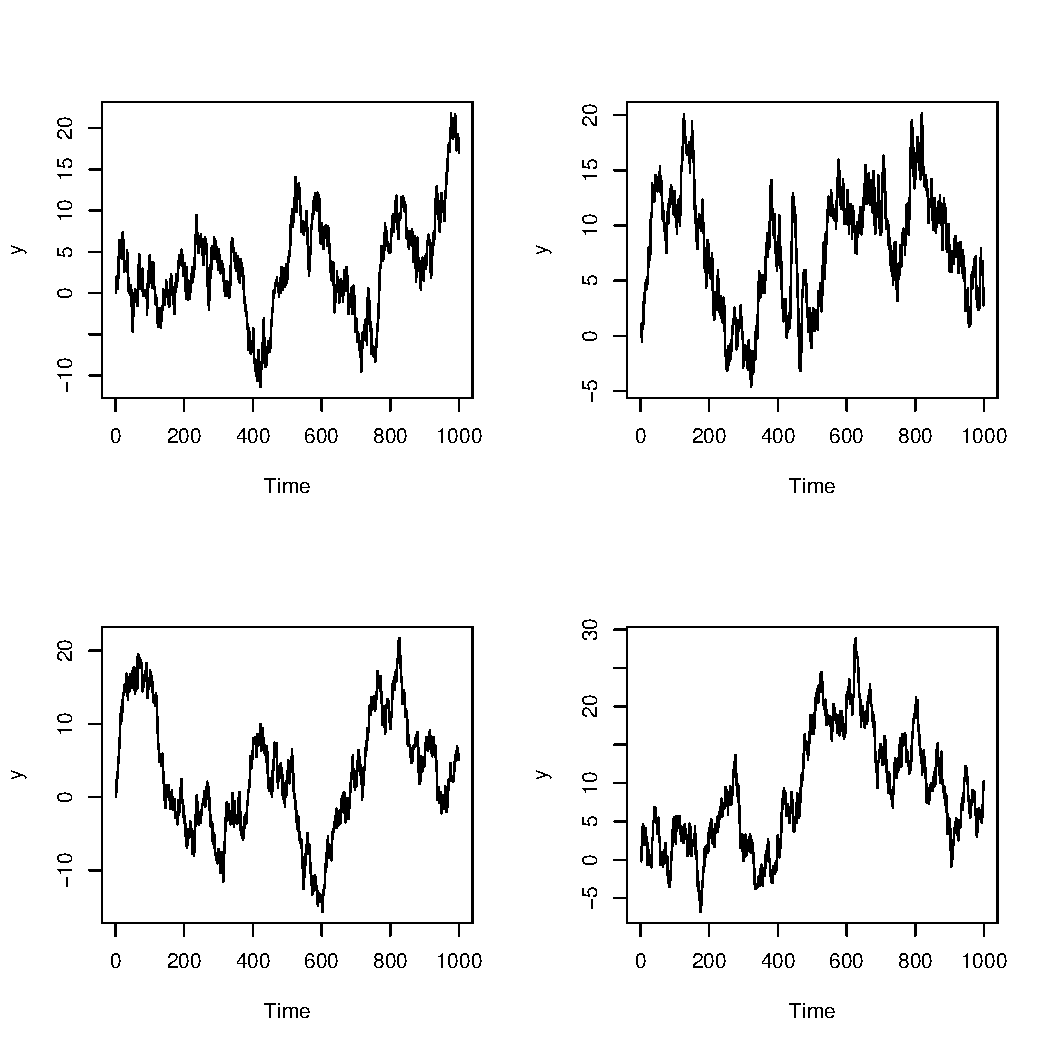
\includegraphics[width=0.6\textwidth]{images/ar1.pdf}
\end{center}

\end{frame}


\begin{frame}[fragile]
\frametitle{Mystery Data}
\begin{center}
\includegraphics[width=0.6\textwidth]{images/nzd.pdf}
\end{center}

\end{frame}


\end{document}

